\documentclass[tikz]{standalone}
\usetikzlibrary{arrows.meta}
\begin{document}

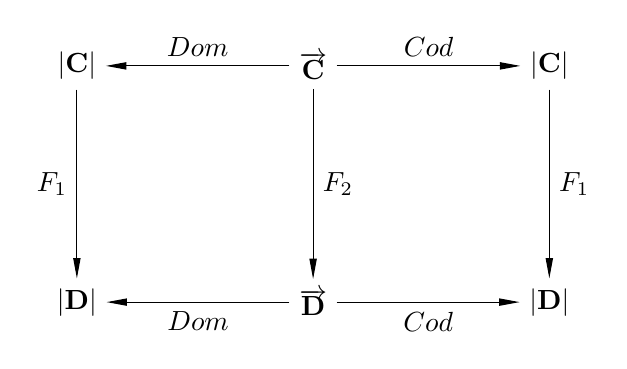
\begin{tikzpicture}[-latex, arrows={-Triangle[angle=20:5pt,scale=1.5]}]
	\node (O1) at (0,0) {\(\overrightarrow{\mathbf{C}}\)};
	\node (O2) at (0,-3) {\(\overrightarrow{\mathbf{D}}\)};

	\node (C1) at (-3,0) {\(| \mathbf{C} |\)};
	\node (C2) at (3,0) {\(| \mathbf{C} |\)};

	\node (D1) at (-3,-3) {\(| \mathbf{D} |\)};
	\node (D2) at (3,-3) {\(| \mathbf{D} |\)};

	\draw (O1) to node [above] {\(Dom\)} (C1);
	\draw (O1) to node [above] {\(Cod\)} (C2);
	\draw (O2) to node [below] {\(Dom\)} (D1);
	\draw (O2) to node [below] {\(Cod\)} (D2);

	\draw (O1) to node [right] {\(F_2\)} (O2);
	\draw (C1) to node [left] {\(F_1\)} (D1);
	\draw (C2) to node [right] {\(F_1\)} (D2);

\end{tikzpicture}

\end{document}
